Database designet er en todelt affære. Delingen er mellem selve strukturen af databasen og koden som tilgår databasen.
Disse beskrives begge i følgende afsnit.

\subsubsection{Database Opbygning}
Opbygningen af den fysiske database er sket ved at opstille designet via et \gls{DSD}. Systemets \gls{DSD}  kan ses på figur~\ref{fig:DSD}. Ud fra diagrammet er det muligt at eksportere SQL kode vha. \gls{DDS-Lite} og derved realisere designet. Koden kan derefter bruges til at opsætte et ''SQL Server Database Project'' i Visual Studio. 

\begin{figure}[H]
    \centering
    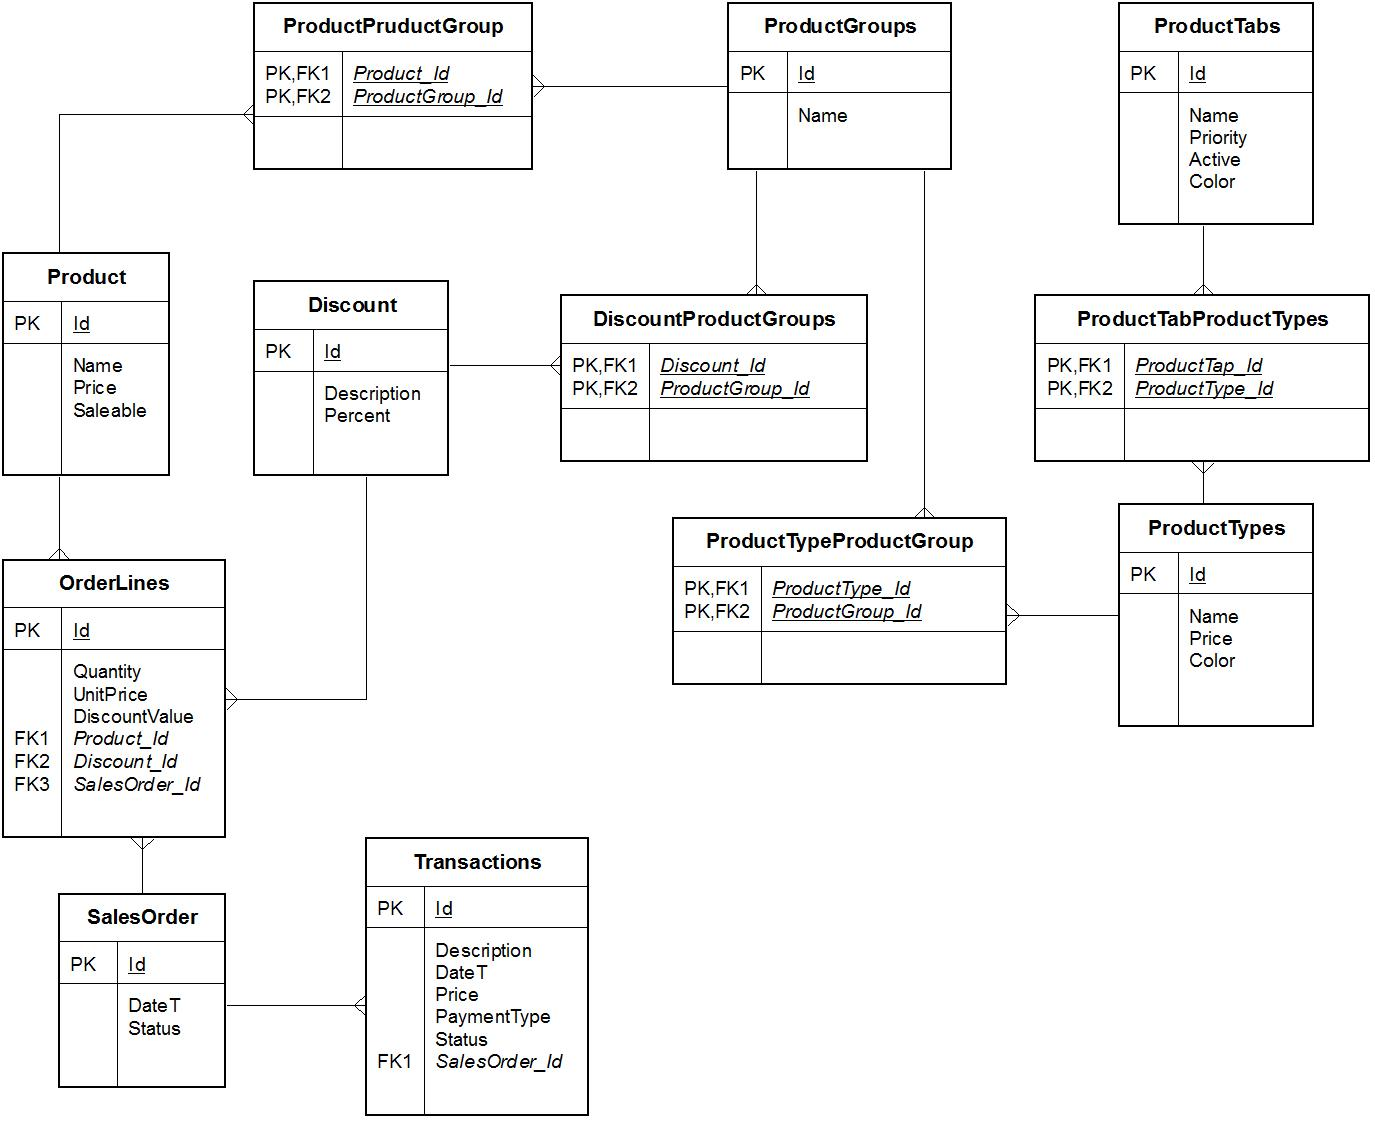
\includegraphics[width=0.6\textwidth]{N+1/DataView/DabDSD}
    \caption{\gls{DSD} over databasen}
    \label{fig:DSD}
\end{figure}

Databasen er designet ud fra følgende tankegang:
\begin{itemize}
	\item Et salg kan have flere salgsbestillinger
	\item Et salg kan betales med flere transaktioner
\end{itemize}
I databasen indeholder tabellen \textit{SalesOrder} alle salg, \textit{OrderLines} alle salgsbestillinger og \textit{Transactions} alle transaktioner. Disse tabeller har et relationship. Ud fra tankegangen skal \textit{SalesOrder} have et \textit{One-to-Many} forhold til \textit{OrderLines} og \textit{Transactions}. Der kan læses mere om database designet i DataView i systemarkitekturdokumentet.
\newline\newline
\textit{OrderLines} bruges til at definere, hvor meget af et \textit{Product}, som er blevet solgt, og hvor meget produktet er solgt til. Hvis der er givet en \textit{Discount}, angives denne også med, hvor meget rabat, som er givet på det enkelte produkt. \textit{Discount} kan være tom, hvis der ikke er givet nogen rabat.
\newline\newline
figur~\ref{fig:DSD} udstiller også \textit{ProductGroups}, \textit{ProductTypes} og \textit{ProductTabs}. \textit{ProductGroups} bruges til at gruppere produkter i grupper som f.eks. sodavand og drinks. Denne har et \textit{Many-to-Many} forhold til \textit{Product} og \textit{Discount}, fordi et \textit{Product} kan have flere \textit{ProductGroups}, og en \textit{Discount} kan tilhører flere \textit{ProductGroups}. \textit{ProductTypes} bruges til at gruppere \textit{ProductGroups} i samme priskategori og derved give dem en ens farve på \gls{brugergraenseflade}n. \textit{ProductTabs} bruges til at definere hvilke tabs, som kan ses på \gls{brugergraenseflade}n. \textit{ProductTabs} kan indeholde mange \textit{ProductTypes}.

\subsubsection{Database kode}
For at kunne tilgå databasen fra systemet blev der brugt \gls{EF}. 
Der blev brugt ''Code First from Existing Database'' i Visual Studio til at danne \gls{EF} modeller, da designet af databasen var lavet i forvejen. Derved afspejler objekterne den allerede designede model, som det kan ses i figur~\ref{fig:CodeFirstFromDB}. Denne metode virkede til første iteration af databasen, men det viste sig herefter at være lettere at få \gls{EF} til at bygge databasen udfra koden, hvis der blev foretaget ændringer.

\begin{figure}[H]
    \centering
	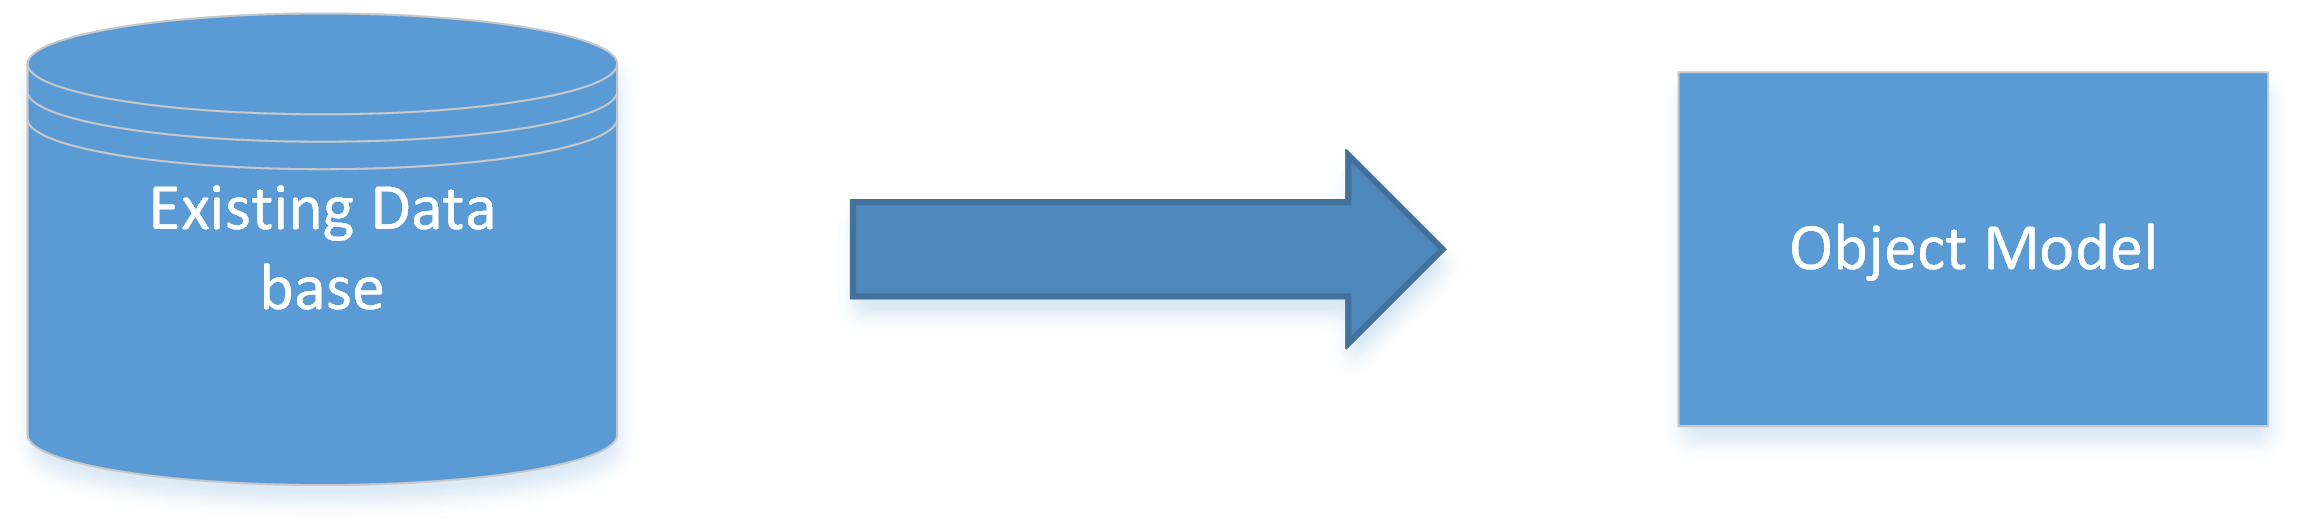
\includegraphics[scale=1]{Rapport/EFCFFDB.PNG}
	\caption{Forbindelse mellem objekter og model}
	\label{fig:CodeFirstFromDB}
\end{figure} 

I systemet blev \gls{EF} pakket ind i \gls{DAL}. Dette blev brugt til at adskille framework koden fra systemet. Denne designmæssige beslutning betyder, hvis systemet skal skifte \gls{EF} ud, er \gls{DAL} det eneste lag, som skal ændres.
\newline\newline
\gls{DAL} består af tre klasser: en \texttt{DALFacade}, et \texttt{UnitOfWork} og et \texttt{Repository}. 
\texttt{DALFacade} bruges til at sørge for, at der kun findes et \texttt{UnitOfWork} ad gangen.
\texttt{UnitOfWork} er en samling af \texttt{Repository}'s, som kan tilgås alt efter hvilken information, som skal bruges. Når der skal ændres noget i et \texttt{Repository} er det \texttt{UnitOfWork}'s opgave at sørge for at der bliver kaldt ''Save'' på \gls{EF}'s \textit{context}.
Et \texttt{Repository} indeholder metoder til at udføre \textit{Create}, \textit{Read}, \textit{Update} og \textit{Delete} af information.
